\documentclass[letter]{article}
\usepackage{graphicx}
\usepackage[margin=2cm]{geometry}
\usepackage{siunitx}

% Try to edit this document such that each sentence starts on its own
% line in order to help with git merge/diff/etc.
%  If you use Emacs, this will help:
% http://stackoverflow.com/questions/539984/


\usepackage{xspace}
\usepackage{bbm}                %Debian/Ubuntu package texlive-fonts-extra

\newcommand\fixme[1]{\textbf{FIXME:} \textit{#1}\xspace}

%% define some of the formal terms
\def\mQraw{Q^{\mathrm{raw}}_{t,i}}
\def\Qraw{$\mQraw$\xspace}

\def\mQdec{Q_{t,i}}
\def\Qdec{$\mQdec$\xspace}

\def\mQexp{Q^{\mathrm{exp}}_{t,i}}
\def\Qexp{$\mQexp$\xspace}

\def\mQmeas{Q^{\mathrm{meas}}_{t,i}}
\def\Qmeas{$\mQmeas$\xspace}

\def\mVcov{V_{t,ij}}
\def\Vcov{$\mVcov$\xspace}

\def\mAchc{A_{i\alpha}}
\def\Achc{$\mAchc$\xspace}

\def\mAchw{A^{\mathrm{chw}}_{ia}}
\def\Achw{$\mAchw$\xspace}

\def\mAwc{A^{\mathrm{wc}}_{a\alpha}}
\def\Awc{$\mAwc$\xspace}

\def\mQcell{Q^{\mathrm{cell}}_\alpha}
\def\Qcell{$\mQcell$\xspace}

\title{Wire Cell Method for LArTPC Reconstruction}
\author{Wire Cell Development Team\\Electronic Detector
  Group\\Physics Department\\Brookhaven National Lab\\(DRAFT, NOT (yet) FOR DISTRIBUTION)}

\begin{document}
\maketitle

\section{Overview}

\fixme{Section to be written to cover the following:}

\begin{itemize}
\item Brief description of the physics relevant to LAr TPC detectors
  with wire readout (ionization, drift, field, induction/collection,
  optical system to measure event time).
\item Brief description of the confounding aspects of LAr TPC
  (degeneracy of three 1D readouts of a 2D space, confounding
  ambiguity due to wire wrapping, the convoluted signal and detector
  response, what eles?)
\item Traditional approach.
\item Name this method: ``Wire Cell''
\item Briefly describe how it differs from traditional, reference
  section~\ref{sec:method} for details.
\end{itemize}

\section{Terms}

\fixme{This section should be removed for a real paper and the terms
  should be defined on first use.}

This section defines general and formal terms used in the document and
the software.
In conversation, please try to all use the same general terms.

\subsection{General Terms}

Specific terms used in this document and the software.

\begin{description}
\item[conductor] one contiguous run of a long thin conducting cylinder  
\item[wire] a single span of a \textit{conductor} strung across the drift
  volume perpendicular to the drift direction.
  AKA \textit{wire segment}.
  Some detectors may have multiple wires for any given single
  conductor due to wrapping the conductor around the wire frame.
\item[wire plane] a hypothetical plane containing all \textit{wires} which run
  parallel to each other.
  All three \textit{wire planes} are parallel.
\item[signal] voltage as a function of time on a \textit{conductor}
\item[channel] a connection of a \textit{conductor} to electronics
  which digitizes a voltage on the conductor as a function of time.
\item[deconvolution] the process by which a digitized \textit{signal} is
  transformed to remove the systematic effect of the
  induction/collection response and which may impart residual
  systematic smearing.
  (Currently this is performed external to this package.)
\item[charge] a measure of the \textit{signal} voltage integrated over
  some time bin.
\item[trace] representation of \textit{charge} and
  time information about a \textit{signal} after deconvolution.
  In general a \textit{trace} may represent part of an entire
  \textit{signal}.
  (Eg: zero-suppression or other thresholds can lead to multiple
  \texttt{traces} being associated to one channel when before there
  was but one.)
\item[cell] a region of the plane parallel to the \textit{wire planes}
  which is spatially associated with a number of \textit{wires} from
  each \textit{wire plane}.
\item[tiling] a collection of \textit{cells} which tile the plane.
\item[slice] a selection of a portion of each \textit{trace} in a
  collection of \textit{traces} which covers the same, contiguous
  region of their time bins.
\item[frame] a collection of \textit{traces} which are contiguous with
  respect to data acquisition, deconvolution and formation of
  \textit{slices} (aka a detector ``event'' or ``trigger'').
\end{description}

\subsection{Formal Terms}

These terms are used to formally describe the problem and have
analogues in the software.
Note, the vectors and matrices involved may very large ($10^4$ wires
and $10^7$ cells in a MicroBooNE geometry) so naive vector/matrix
representations are not used in the software.

\noindent The indices are chosen to indicate as in:
\begin{description}
\item[$t$] a time bin.
  This same indication is used be it a raw digitized time bin, a time
  bin after deconvolution or a possibly aggregate time bin produced by
  a slice.
\item[$a,b,c$] Latin indices in this range are used to enumerate \textit{wires}.
\item[$i,j,k$] Latin indices in this range are used to enumerate \textit{channels}.
\item[$\alpha,\beta$] Greek indices are used to enumerate \textit{cells}.
\end{description}

\noindent The formal terms used in this problem are:
\begin{description}
\item[\Qraw] the digitized \textit{charge} on channel $i$ at
  time bin $t$.
\item[\Qdec] the \textit{measured channel-charge vector} which gives the measured \textit{charge} on channel $i$ at
  time bin $t$ after deconvolution has been applied.
\item[\Qexp] an estimator or expected value of the above.
\item[\Vcov] a covariance matrix giving the 
  uncertainty in the \Qdec measurements at time $t$ between channels
  $i$ and $j$.
  This matrix is $n_\mathrm{channels}$-rows by $n_\mathrm{channels}$-columns.
\item[\Achc] the matrix representing the association between \textit{channels} and {cells}.
  It is a product of the following two matrices.
  This matrix is $n_\mathrm{channels}$-rows by $n_\mathrm{cells}$-columns.
\item[\Achw] the matrix representing the association between
  \textit{channels} and \textit{wires}.
  This matrix is $n_\mathrm{channels}$-rows by $n_\mathrm{wires}$-columns.
\item[\Awc] the matrix representing the association between
  \textit{wires} and \textit{cells}.
  This matrix is $n_\mathrm{wires}$-rows by $n_\mathrm{cells}$-columns.
\item[\Qcell] the \textit{cell-charge} vector representing the charge passing
  through a \texttt{cell} in a given time bin $t$.
\end{description}

\section{Method}

The goal of this method is to reconstruct the two dimensional pattern
of charge drifting through the wire planes at given time.
This section describes the general method employed to reach
this goal and some formalism describing its procedures.
Subsequent sections describe implementation and optimization details
which exploit an understanding of expected classes of LAr TPC event topology.

At a high level, the wire-cell method follows these broad steps:

\begin{enumerate}
\item Form a \textit{tiling} of \textit{cells} that associate \textit{channels} with a 2D
  region of nearly-crossing \textit{wires} (\Achc matrix)
\item Use information in the \textit{slice} to reduce the size of
  \Achc in a information-lossless manner.
\item Attempt to solve for the cells in terms of the channels (described below)
\item If initial solution fails, try a number of information-lossy
  methods to further reduce the size of \Achc (described below)
\end{enumerate}

\section{Tiling}

A hypothetical plane parallel to and approximately coplanar with the
\textit{wire planes} is partitioned into \textit{cells} via a
\textit{tiling} process.
In general, a tiling produces an associative mapping from localized
regions of the plane to the wires which pass through the region or, by
some metric, near by.
Multiple tiling methods are conceivable and result in different
associations.
These different methods are described later in this section.

A potential tiling must satisfy some general criteria:

\begin{enumerate}
\item It must produce ``small'' cells with sizes comparable to wire pitch
   (in order to not lose spatial resolution).
 \item It associates a cell with at least one wire from each plane.
 \item It supports the various queries needed (eg, cell-wire and
    wire-cell look-ups)
\end{enumerate}

The wire-cell association of an arbitrary tiling can be represented as
a \textit{bipartite graph} with $N_{wires}$ vertices representing the
wires and $N_{cells}$ vertices representing the cells.
As such it can also be represented as a $N_{wires} \times N_{cells}$
association or \textit{biadjacency} matrix or as a block-off-diagonal
square \textit{adjacency matrix} of size $N_{wires} + N_{cells}$.
Below we use the \textit{biadjacency} representation but refer to the
graph representation at times.
Elements in this association matrix \Awc are zero if a wire and a cell
are not associated.
A non-zero element may be unity or may be some number $<1$ if the
association is weighted.

It is noted that DUNE detectors employ ``wire wrapping'' such that
they have an $N \to 1$ mapping from \textit{channel} to
\textit{wires}.
The solving for ``hit'' \textit{cells} described below require a ($N
\to M$) mapping from \textit{channels} to \textit{cells} and the
tiling is just one factor of that mapping.
Taking this to account, a full mapping from the number of hits in a
cell to their measured charge in associated channels is the
\textit{channel-cell matrix}.

\begin{equation}
  \label{eq:Achc}
  \mAchc = \mAchw \mAwc
\end{equation}

For detectors with no wire wrapping $\mAchw \equiv \mathbbm{1}$.
Given knowledge of the charge in a cell at a given time one can write
the (deconvolved) charge expected to be measured in channel $i$ at
time $t$ as

\begin{equation}
  \label{eq:Qexp}
  \mQexp = \mAchc \mQcell.
\end{equation}

In the absence of uncertainties, the \textit{expected} channel-charge vector \Qexp
can be identified with the \textit{measured} channel-charge vector \Qmeas and the
channel-cell matrix \Achc can be potentially inverted and thus one may solve
for the cell-charge vector.
However, there are two confounding problems to performing this
inversion which are described in
subsection~\ref{subsec:tilingdegeneracy} and section~\ref{sec:chargeunc}.

\subsection{Tiling Algorithms}
\label{subsec:tilingalg}

This section describes some tiling algorithms that are being considered.
The general approach of the wire-cell method is expected to be
somewhat independent from the exact tiling procedure.
It is expected that some tilings will perform differently in terms of
spatial resolution and computational speed.

Figure~\ref{fig:eyeball} shows some examples of wire patterns from
existing detectors and ones being designed.

\begin{figure}[htbp]
  \centering

  \begin{minipage}[b]{0.3\linewidth}
    \begin{center}
        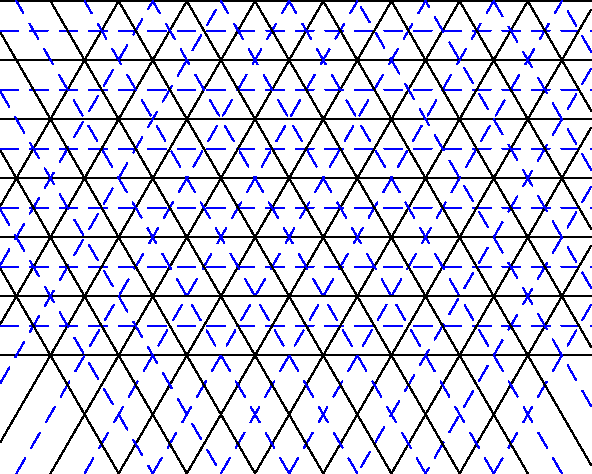
\includegraphics[width=\textwidth]{wires-uboone.pdf}              

        MicroBooNE
    \end{center}
  \end{minipage}
  \begin{minipage}[b]{0.3\linewidth}
    \begin{center}
        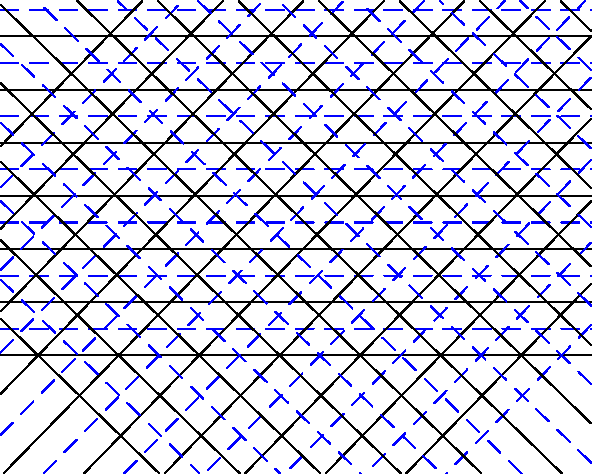
\includegraphics[width=\textwidth]{wires-35t.pdf}      

        DUNE \SI{35}{\tonne}
    \end{center}
  \end{minipage}
  \begin{minipage}[b]{0.3\linewidth}
    \begin{center}
        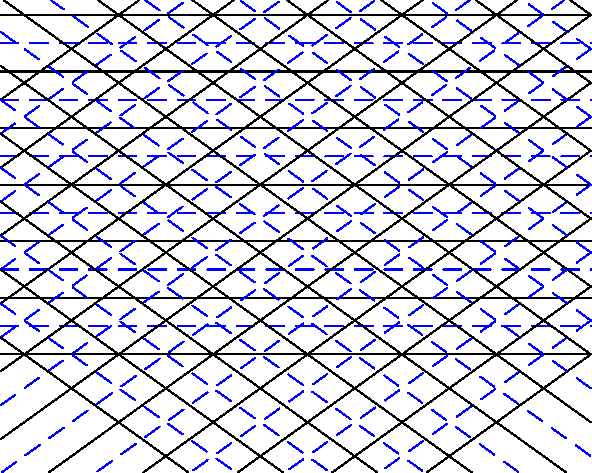
\includegraphics[width=\textwidth]{wires-10kt.pdf}              

        DUNE \SI{10}{\kilo\tonne}
    \end{center}
  \end{minipage}

  \caption{Wire patterns (black lines) and their half-way lines (blue,
    dashed) for MicroBooNE (left), DUNE \SI{35}{\tonne} prototype detector
    (center) and DUNE \SI{10}{\kilo\tonne} far detector (right).
  Between figures, wire pitches are not to scale.}
  \label{fig:eyeball}
\end{figure}

\subsubsection{Trivial Tiling}

The most trivial tiling is built by first identifying the
\textit{half-way lines} the run midway between and parallel to any two
neighboring wires in the same plane.
The complete family of these lines produce the same pattern as the
wires themselves but are offset by $\frac{1}{2}$ of a wire pitch in
the direction transverse to the wire plane.
The trivial tiling then identifies each smallest polygon bound by
half-way lines and which has no other half-way lines intersecting.

The tiling can be thought of as a cyclical, undirected graph made of
nodes formed by the crossing points of half-way lines and edges made
by the connecting of these points by the half-way lines themselves.

To identify the cells the following algorithm can be used.
Place all nodes in a sequence.
Pop the first node from that sequence, call this the seed.
Form a collection of groups (initially pairs) with the seed and every node directly
connected via the seed's edges.
Call each of these nodes the ``tail'' of the group.
Iterate on the remaining sequence and
for each node, add it as a new ``tail'' node if it is connected to an
existing tail node via an edge.
Determine if the same node was added to twice to any group,
identify those two groups as surrounding the cell and remove them from
the collection of groups.
After this iteration all cells containing the original seed are found.
Repeat with the next node in the sequence. 

\subsubsection{Bounded Tiling}

Bounded tiling is simple and fairly fast if order $N^3$ in the number
of wires.
For each U and V wire determine the four crossing points of their
half-way lines.
Then, for each Y wire, find its half-way lines and determine if any of
the four U/V crossing points are bound between them.
If so, save them and find the crossing points of the Y-half-way lines
and the U-half-way lines and if they are bound by the two V-half-way
lines save them.
Repeat to determine if any Y and V crossings are bound by the
U-half-way lines.
All crossings of pairs of half-way lines from two planes which are
bound by half-way lines of the third plane are thus included in the cell.


\subsubsection{Minimum Association}

\fixme{Michael, fill this in, for now, it's just my blah blah.
Also, let's pick a better name.}

This section describes Michael's algorithm.
It assigns exactly one wire from each plane to a cell.
For the regular MicroBooNE wires the cells produced fall into two
categories: regular hexagon shape and regular isosceles triangles of 
$\frac{1}{6}$th size of the hexagons.



\subsubsection{UV Diamond}

The UV Diamond tiling simply identities a cell as the diamond-shaped
region bounded by the half-way lines of the U and V wires.
Such cells are centered on U-V wire crossing points.

A Y wire is then associated with a UV Diamond cell by determining what
fraction of the cell the band formed by its half-way lines subtend the
cell's area.
This fraction is then used to form a weighted association matrix.

This tiling reflects the symmetry that exists in the fact
that U and V wires record induced charge while the Y wires record
collected charge.
It also exploits the spatial symmetry that exists when only two wire
planes are considered.
The UV Diamond cells then form a rectilinear space which can be mapped
to Cartesian coordinates.
This facilitates many required procedures such as indexing a cell
given a point in space.

When attempting to remove tiling degeneracy (see
section~\ref{subsec:tilingdegeneracy}) this construction can help in a
few ways.
One may elect to sever wire-cell associations based on some selection
criteria on the association weight.
This would be done independent from any measured charge patterns, but
measured charge could be used in a similar manner to break
associations based on the weighted change each wire contributes to a cell.
Such operations will likely require heuristics to be developed based
on actual wire patterns and expected event topology.


\subsection{Tiling Degeneracy}
\label{subsec:tilingdegeneracy}

For realistic cases, it is not possible to invert the full
channel-cell matrix in because of its inherent degeneracy.
It maps approximately $3N$ ``knowns'' (channel measurements) to $N^2$
``unknowns'' (cells) where $N$ here is a number of order the number of
wires in one plane ($\sim 10^3$).
The size alone poses a practical problem due to system memory and CPU
usage.
Strategies to approach reducing the size of the channel-cell matrix
are described in section~\ref{sec:reduction}.
These procedures will either identify certain channels or cells which
may be removed from consideration or which may be effectively joined
or merged.

\subsection{Tiling Translational Invariance}

One feature of a particular tiling which can help in reducing memory
usage is if it has any step-wise translational invariance.
If the tiling repeats over some distance it may be possible to
represent the tiling in a compact way by storing only the
non-repeating region.

The MicroBooNE case is trivial.
Wire crossings form a regular lattice made of isosceles triangles and
tilings can be formed which repeat at a distance equal to that between
any two neighboring, triple-crossing points.

DUNE detectors are less regular due to engineering constraints.
The DUNE 35t detector is least regular in that the U and V wires each have
differing angles with respect to the Y wires.
The other DUNE detectors are designed to have identical U and V angles
(opposite signs)
but are chosen such that they may not produce a regular pattern with
respect to the Y wires.
\fixme{Actually check this statement.}


The translational invariance condition can be described in the
following manner.
First, without loss of generality, one can imagine shifting the Y wire
play in a direction orthogonal to its wires so that one can form at
least one triple-wire crossing between a Y, a U and a V wire.
If the pattern of wires repeat then from that point one can imagine
forming a vector to another triple-wire crossing which occurs such
that the pattern from this new point is invariant to the pattern from
the original.

The condition of that point is:

\begin{equation}
  \label{eq:transinvcond}
  n_y*P_y = n_v v \sin(\theta_v) + n_u u \sin(\theta_v)
\end{equation}

Where the $n_y$ etc are integers, $P_y$ is the wire pitch of the Y
wires, $v$ and $u$ measure the distance along the V and U wires
between U/V intersection points and $\theta_v$ and $\theta_u$ are the
angles of V and U wires with respect to the Y wires.
\fixme{I did this
  on the plane and it still needs checking!}
  
Then, if integers $n_y$, etc, can be found which satisfies this
equation, the cell pattern repeats as given by the vector formed using
their values and the known wire directions.
The magnitude of this vector may be larger than the physical extent of
the detector, in which case the no exact reduction in the size of the
representation of the tiling is possible.
It may be possible to approximately satisfy
equation~\ref{eq:transinvcond} such that errors in the approximation
are small compared to the wire pitches across the entire physical extent.



\section{Measurement Uncertainty}
\label{sec:chargeunc}

The second problem that confounds inverting the channel-cell matrix,
even after it is reduced as above, is that this matrix alone does not
account for the uncertainty that exists in the measured charge.
This uncertainty is potentially covariant among the channels and thus
leads to an additional, effective mixing between channels and cells
beyond the multiplexing which is inherent in the definition of the
tiling.
The sources of measurement uncertainty fall into categories including
noise which may be correlated or uncorrelated between the channels and
residual smearing in time from the deconvolution process.

In order to incorporate this uncertainty the expected channel charge
vector (eqn~\ref{eq:Qexp}) is compared against its measured equivalent and 
a $\chi^2_t$ value is formed

\begin{equation}
  \label{eq:chi2}
  \chi^2_t(\mQcell) = (\mQdec - \mQexp)^\mathsf{T}\mVcov^{-1}(Q_{t,j} - Q^{\mathrm{exp}}_{t,j})
\end{equation}

\noindent Minimizing with respect to \Qcell gives,

\begin{equation}
  \label{eq:Qcell}
  \mQcell = [(A^\mathsf{T}V_t^{-1}A)^{-1}]_{\alpha\beta}
  (A^\mathsf{T}V_t^{-1})_{\beta i}\mQdec
\end{equation}
Where indices internal to some of the matrix products have been
dropped for clarity.

\section{Channel-Cell Matrix Reduction}
\label{sec:reduction}

Again, in eqn~\ref{eq:Qcell}, the Latin indices run over
channels and the Greek over cells.
One rough estimate of the number of cells to be defined in any given
detector is,
\begin{equation}
  \label{eq:ncellsestimate}
  N_\mathrm{cells} \approx N_\mathrm{wires}^2/9
\end{equation}

This ignores wire wrapping (increases number of cells per channel) and
assumes the same number of wires per plane and that the number of
cells can be estimated assuming every wire from one plane crosses
every wire from another plane and further that there is one cell per
crossing.
Table~\ref{tab:detectorcounts} gives channel counts and estimates for the
number of cells and the size of the full channel-cell matrix.

\begin{table}[htbp]
  \centering
  \begin{tabular}[h]{|r|r|l|l|}
    \hline
    Detector & \#channels & \#cells & $size(\mAchc)$ \\
    \hline
    \hline
    % fixme: 512 is per face or per all APA?
    DUNE 35t APA Face & 512/2 & $7\times 10^3$ & $2\times 10^6$\\
    DUNE 10kt APA Face & 2560/2 & $2\times 10^5$ & $2\times 10^8$ \\
    MicroBooNE & 8256 & $7\times 10^6$ & $6\times 10^{10}$\\
    \hline
  \end{tabular}
  \caption{Channel counts and estimated number of cells of some LAr
    TPC detectors.
    In the case of DUNE detectors, only one APA (face) is considered
    and wire wrapping is ignored.
    Wire wrapping will approximately double the number of cells.
    A single 10kt DUNE module (1 of 4) will have 150 APAs sensing 200 LAr drift regions.}
  \label{tab:detectorcounts}
\end{table}

\subsection{Reduction Matrix}

The size of the matrices given in Table~\ref{tab:detectorcounts} as
well as the inherent tiling degeneracy requires some procedures to
reduce the size of the problem.
One way to represent such procedures is to introduce the idea of
\textit{reduction matrices}.


As described in more detail in the following sections, the nature of
the reduction procedures can grouped into two categories: removal or
merging or channels or cells.

A removal is represented by constructing a series of
\textit{row-switching} transformation matrices.
These are square matrices of size $N_{ch}$ or $N_{cells}$ depending on
which basis they operate.
The inverse of such matrices are themselves and so as many pairs may
be inserted as needed to move a given row to the last row of the matrix.
A basis can then be truncated to produce a smaller matrix equation.

A merge is a transformation where two elements becomes logically one.
For example, a merged cell is a new logical cell which has associated
all wires of its constituent cells.
A merge is represented by a \textit{row-addition} transform matrix
which is the identity pull an entry at $\delta_{ij}$.
It's inverse is simply the same matrix but with the extra entry $-\delta_{ij}$.
The effect is that elements at index $i$ become the sum of elements at
$i$ and $j$.
A removal transform is inserted to remove the entry at $j$.

In general a reducing operation consists of applying or inserting a
series of the transformation matrices (and possibly paired with their
inverse) described above into a given equation.
We represent their product-series as an overall reduction matrix
$R^{ch}$ if it operates on the channel basis and $R^{cell}$ if on the
cell basis.
As an example, applying a channel reduction and inserting a cell
reduction to eqn~\ref{eq:Qexp} gives:

\begin{equation}
  \label{eq:contraction}
  R^\mathrm{ch} Q^\mathrm{exp}_t = 
R^\mathrm{ch} 
A (R^\mathrm{cell})^{-1} 
R^\mathrm{cell}  
Q^\mathrm{cell}
\end{equation}

\noindent It is then clear that the same formula is retained with the
substitution:

\begin{equation}
  \label{eq:subst}
  R^\mathrm{ch} A (R^\mathrm{cell})^{-1} \to A\\
\end{equation}
\begin{equation}
  \label{eq:subst2}
  R^\mathrm{x} Q^\mathrm{x} \to Q^\mathrm{x}
\end{equation}

\subsection{Lossless Reduction}

Some channels may not provide any contribution to the charge in a
given slice.
These channels may be removed in order to reduce the size of the
matrices in an information-lossless manner.
Such channels may come about due to the time bin for that channel failing to
satisfy zero-suppression (ZS) threshold applied during DAQ readout or
an analysis threshold applied offline.

\subsection{Lossy Reduction}

In general a time slice can not be solved after lossless reduction.  Further
reduction is attempted which is information-lossy in nature but which
is hoped to reduce the complexity enough to allow solving the slice. 


\subsubsection{Blobs}

After lossless reduction of a time slice, one is left only with
channels containing charge and all their associated cells which are
considered to be \textit{potentially hit} in that they all potentially
contained drifting charge.
Using the geometrical locations of these cells it is possible to merge
neighboring cells into a number groups termed ``merged cells'' or
``\textit{blobs}''.

The extent and location of a blob is well defined in the 2D drift
plane however in any given wire plane individual blobs may appear to
overlap.
One can construct a bipartite graph between blobs and their associated
channels in a single wire plane.
If this graph is composed of a number of fully connected subgraphs
then that wire plane gives some individual measurement of a subset of
the blobs.
Combining these measurements in the three views may allow for the
amount of charge in each blob to be calculated.


\subsubsection{Inter-slice Interpolation}

Another approach is to delay solving a slice until solutions are
achieved for the two slices which
bracket in time the unsolved one.
With the pair of solved slices in hand one may apply some inter-slice
interpolation for cells found problematic, remove their contribution
from the associated wires and attempt to re-solve.
Or, one may perform a $\chi^2$ fit using eqn~\ref{eq:chi2} using the
bracketing slices to direct the search space. 

\subsubsection{Kinematic Fitting}
t.b.d.

\end{document}
